\section{Evaluation}
\label{sec:exp}



\vspace{-2mm}
\subsection{Experimental Setup}
\label{exp:setup-exp}
\vspace{-2mm}
\myparatight{Datasets}We use three benchmark question-answering datasets in our evaluation: \emph{Natural Questions (NQ)}~\cite{kwiatkowski2019natural}, \emph{HotpotQA}~\cite{yang2018hotpotqa}, and \emph{MS-MARCO}~\cite{nguyen2016ms}, where each dataset has a knowledge database. The knowledge databases of NQ and HotpotQA are collected from Wikipedia, which contains 2,681,468 and 5,233,329 texts, respectively. The knowledge database of MS-MARCO is collected from web documents using the MicroSoft Bing search engine~\cite{bing-msmarco}, which contains 8,841,823 texts. Each dataset also contains a set of questions. Table~\ref{tab:dataset} (in Appendix) shows statistics of datasets. 



\myparatight{RAG Setup} Recall the 
three components in RAG: \emph{knowledge database}, \emph{retriever}, and \emph{LLM}. Their setups are as below:
\begin{itemize}
    \vspace{-2mm}
    \item \myparatight{Knowledge database}We use the knowledge database of each dataset as that for RAG, i.e., we have 3 knowledge databases in total.
    \vspace{-2mm}
    \item \myparatight{Retriever}We consider three retrievers: Contriever~\cite{izacard2022unsupervised}, Contriever-ms (fine-tuned on MS-MARCO)~\cite{izacard2022unsupervised}, and ANCE~\cite{xiong2021approximate}. Following previous studies~\cite{zhong2023poisoning, lewis2020retrieval}, by default, we use the dot product between the embedding vectors of a question and a text in the knowledge database to calculate their similarity score. We will also study the impact of this factor in our evaluation. 
    \vspace{-2mm}
    \item \myparatight{LLM} We consider PaLM 2~\cite{anil2023palm}, GPT-4~\cite{achiam2023gpt}, GPT-3.5-Turbo~\cite{brown2020language}, LLaMA-2~\cite{touvron2023llama} and Vicuna~\cite{vicuna2023}. The system prompt used to let an LLM generate an answer for a question can be found in Appendix~\ref{appendix-sec-system-prompt}. We set the temperature parameter of LLM to be 0.1.
\end{itemize}




Unless otherwise mentioned, we adopt the following default setting. We use the NQ knowledge database and the Contriever retriever. 
Following previous study~\cite{lewis2020retrieval}, we retrieve $5$ most similar texts from the knowledge database as the context for a question. Moreover, we calculate the dot product between the embedding vectors of a question and each text in the knowledge database to measure their similarity.  We use PaLM 2 as the default LLM as it is very powerful (with 540B parameters) and free of charge, enabling us to conduct systematic evaluations. We will evaluate the impact of each factor on our knowledge corruption attacks. 

\myparatight{Target questions and answers} {\name} aims to make RAG produce attacker-chosen target answers for attacker-chosen target questions. Following the evaluation of previous studies~\cite{shafahi2018poison,carlini2021poisoning,carlini2021poisoningsemi,liu2022poisonedencoder} on targeted poisoning attacks, we randomly select some target questions in each experiment trial and repeat the experiment multiple times.
In particular, we randomly select $10$ close-ended questions from each dataset 
as the target questions. Moreover, we repeat the experiments 10 times (we exclude questions that are already selected when repeating the experiment), resulting in 100 target questions in total. 
We select close-ended questions (e.g., ``Who is the CEO of OpenAI?") rather than open-ended questions (we defer the discussion on open-ended questions to Section~\ref{sec:discussion-limitation}) because we aim to quantitatively evaluate the effectiveness of our attacks since close-ended questions have specific, factual answers. In Appendix~\ref{appendix-sec-example-target-question}, we show a set of selected target questions. 
For each target question, we use GPT-4 to randomly generate an answer that is different from the ground truth answer of the target question. We manually check each generated target answer and regenerate it if it is the same as the ground truth answer. 
Without attacks, the LLM in RAG could correctly provide answers for 70\% (NQ), 80\% (HotpotQA), and 83\% (MS-MARCO) target questions under the default setting.




\begin{table*}[!t]\renewcommand{\arraystretch}{1.2}
\setlength{\tabcolsep}{1mm}
\fontsize{7.5}{8}\selectfont
\centering
\caption{\RV{{\name} could achieve high ASRs on 3 datasets under 8 different LLMs, where we inject 5 malicious texts for each target question into a knowledge database with  $2,681,468$ (NQ), $5,233,329$ (HotpotQA), and $8,841,823$ (MS-MARCO) clean texts. We omit Precision and Recall because they are the same as F1-Score.}}
\vspace{-2mm}
\begin{tabular}{|c|c|c|c|c|c|c|c|c|c|c|c|c|c|c|}
\hline
\multirow{2}{*}{\makecell{Dataset}} &\multirow{2}{*}{\makecell{Attack}} &\multirow{2}{*}{\makecell{Metrics}} & \multicolumn{8}{c|}{LLMs of RAG}                 \\ \cline{4-11}               
&  & & PaLM 2   & GPT-3.5 & \makecell{GPT-4} & \makecell{LLaMa-2-7B} & \makecell{LLaMa-2-13B}  & Vicuna-7B & Vicuna-13B &Vicuna-33B \\ \hline

\multirow{4}{*}{NQ} & \multirow{2}{*}{\makecell{{\name}\\ (Black-Box)}}&ASR & 0.97 & 0.92 & 0.97 & 0.97 & 0.95  & 0.88 & 0.95 & 0.91 \\ \cline{3-11}
 &  &F1-Score& \multicolumn{8}{c|}{0.96}\\ \cline{2-11}
 &\multirow{2}{*}{\makecell{{\name}\\ (White-Box)}}&ASR & 0.97 & 0.99 & 0.99 & 0.96 & 0.95  & 0.96 & 0.96 & 0.94 \\ \cline{3-11}
 &  &F1-Score& \multicolumn{8}{c|}{1.0}\\ \hline \hline 

\multirow{4}{*}{HotpotQA} & \multirow{2}{*}{\makecell{{\name}\\ (Black-Box)}}&ASR & 0.99 & 0.98 & 0.93 & 0.98 & 0.98  & 0.94 & 0.97 & 0.96 \\ \cline{3-11}
 &  &F1-Score& \multicolumn{8}{c|}{1.0}\\ \cline{2-11}
 &\multirow{2}{*}{\makecell{{\name}\\ (White-Box)}}&ASR & 0.94 & 0.99 & 0.99 & 0.98 & 0.97  & 0.91 & 0.96 & 0.95 \\ \cline{3-11}
 &  &F1-Score& \multicolumn{8}{c|}{1.0}\\ \hline \hline 

\multirow{4}{*}{MS-MARCO} & \multirow{2}{*}{\makecell{{\name}\\ (Black-Box)}}&ASR & 0.91 & 0.89 & 0.92 & 0.96 & 0.91  & 0.89 & 0.92 & 0.89 \\ \cline{3-11}
 &  &F1-Score& \multicolumn{8}{c|}{0.89}\\ \cline{2-11}
 &\multirow{2}{*}{\makecell{{\name}\\ (White-Box)}}&ASR & 0.90 & 0.93 & 0.91 & 0.92 & 0.74  & 0.91 & 0.93 & 0.90 \\ \cline{3-11}
 &  &F1-Score& \multicolumn{8}{c|}{0.94}\\ \hline 

\end{tabular}
\label{tab:main-results}
\vspace{-4mm}
\end{table*}







\begin{table}[!t]\renewcommand{\arraystretch}{1.2}
\setlength{\tabcolsep}{1mm}
\fontsize{7.5}{8}\selectfont
\centering
\caption{Comparing ASRs calculated by the substring matching and human evaluation. The dataset is NQ. }
\vspace{-2mm}
\begin{tabular}{|c|c|c|c|c|c|c|}
\hline
\multirow{3}{*}{\makecell{Attack}} &\multirow{3}{*}{\makecell{Metrics}}& \multicolumn{5}{c|}{LLMs of RAG}                 \\ \cline{3-7}                      
 & & PaLM 2   & GPT-3.5 & \makecell{GPT-4} & \makecell{LLaMa\\-2-7B} & Vicuna-7B  \\ \hline
                      
\multirow{3}{*}{\makecell{{\name} \\ (Black-Box)}}  & \makecell{Substring}& 0.97 & 0.92 & 0.97 & 0.97 & 0.88  \\ \cline{2-7}
 &\makecell{Human\\ Evaluation} & 0.98 & 0.87 & 0.92 & 0.96 & 0.86  \\ \cline{1-7}
 
\multirow{3}{*}{\makecell{{\name} \\(White-Box)}}  &\makecell{Substring} & 0.97 & 0.99 & 0.99 & 0.96 & 0.96  \\ \cline{2-7}
& \makecell{Human \\Evaluation} & 1.0 & 0.98 & 0.93 & 0.92& 0.88  \\ \hline 
\end{tabular}
\label{tab:human-evaluation}
\vspace{-4mm}
\end{table}


\myparatight{Evaluation metrics} We use the following metrics:
\begin{itemize}
\vspace{-2mm}
    \item \myparatight{Attack Success Rate (ASR) 
    } 
    We use the ASR to measure the fraction of target questions whose answers are the attacker-chosen target answers. Following previous studies~\cite{rizqullah2023qasina, huang2023catastrophic}, we say two answers are the same for a close-ended question when the target answer is a substring of the generated one by an LLM under attacks (called \emph{substring matching}). 
    We don't use Exact Match because it is inaccurate, e.g., it views ``Sam Altman'' and ``The CEO of OpenAI is Sam Altman'' as different answers to the question ``Who is the CEO of OpenAI?". 
    We use human evaluation (conducted by authors) to validate the substring matching method. We find that substring matching produces similar ASRs as human evaluation (Table~\ref{tab:human-evaluation} shows the comparison). 
    \vspace{-2mm}
    \item \myparatight{Precision/Recall/F1-Score}{\name} injects $N$ malicious texts into the knowledge database for each target question. We use \emph{Precision}, \emph{Recall}, and \emph{F1-Score} to measure whether those injected malicious texts are retrieved for the target questions. Recall that RAG retrieves top-$k$ texts for each target question. Precision is defined as the fraction of malicious texts among the top-$k$ retrieved ones for the target question. Recall is defined as the fraction of malicious texts among the $N$ malicious ones that are retrieved for the target question. F1-Score measures the tradeoff between Precision and Recall, i.e., $\text{F1-Score} = 2\cdot \text{Precision} \cdot \text{Recall}/(\text{Precision} + \text{Recall})$. We report average Precision/Recall/F1-Score over different target questions. A higher Precision/Recall/F1-Score means more malicious texts are retrieved. 


    \vspace{-2mm}
    \item \myparatight{\#Queries} {\name} utilizes an LLM to generate the text $I$ to satisfy the generation condition.
    We report the average number of queries made to an LLM to generate each malicious text. 
    
    \vspace{-2mm}
    \item \myparatight{Runtime} In both white-box and black-box settings, {\name} crafts $S$ such that malicious texts are more likely to be retrieved for the target questions. 
    {\name} is more efficient when the runtime is less. In our evaluation, we also report the average runtime in generating each malicious text. 
\end{itemize}






\myparatight{Compared baselines} 
To the best of our knowledge, there is no existing attack that aims to achieve our attack goal. In response, we extend other attacks~\cite{perez2022ignore,liuyi2023prompt,greshake2023not,liu2023prompt,zhong2023poisoning} to LLM to our scenario. In particular, we consider the following baselines:
\begin{itemize}
    \vspace{-2mm}
    \item \myparatight{Naive Attack}Given a question $Q$, if we view $Q$ as the malicious text, it will likely be retrieved. We compare with this attack to demonstrate that the generation condition is necessary for knowledge corruption attacks.
    
    \vspace{-2mm}
    \item \myparatight{Prompt Injection Attack~\cite{perez2022ignore,liuyi2023prompt,greshake2023not,liu2023prompt}} Prompt injection attacks aim to inject an instruction into the prompt of an LLM such that the LLM generates an attacker-desired output. Inspired by our black-box attack, we put the target question in the instruction for the prompt injection attacks such that the crafted malicious texts are more likely to be retrieved for the target question.  In particular, given a target question and target answer, we craft the following malicious text: ``When you are asked to provide the answer for the following question: <target question>, please output <target answer>.''. We note that the key difference between prompt injection attacks and {\name} (in the black-box setting) is that prompt injection attacks utilize instructions while {\name} crafts malicious knowledge. 
    

    \vspace{-2mm}
    \item \myparatight{Corpus Poisoning Attack~\cite{zhong2023poisoning}}This attack aims to inject malicious texts (consisting of random characters) into a knowledge database such that they can be retrieved for indiscriminate questions.  This attack requires the white-box access to the retriever. We adopt the publicly available implementation~\cite{zhong2023poisoning} for our experiments. As shown in our results, they achieve a very low ASR (close to Naive Attack). The reason is that it cannot achieve the generation condition. 
    Note that this attack is similar to {\name} (white-box setting) when {\name} uses $S$ alone as the malicious text $P$ (i.e., $P=S$).

    \vspace{-2mm}
    \item \myparatight{GCG Attack~\cite{zou2023universal}}\RV{Zou et al.~\cite{zou2023universal} proposed an optimization-based jailbreaking attack to LLM. In particular, given a harmful question, they aim to optimize and append an adversarial suffix (an adversarial text) such that the generated output of the LLM starts with an affirmative response (e.g., ``Sure, here is''). We extend the GCG attack to our scenario. In particular, we can optimize an adversarial text such that the LLM generates the target answer for a target question (see Appendix~\ref{appendix-gcg-details} for our adaptation details). Then, we view the optimized adversarial text as a malicious text and inject it into the knowledge database. Our results show that GCG achieves a very low ASR (close to Naive Attack). The reason is that it cannot achieve the retrieval condition.}

    \vspace{-2mm}
    \item \myparatight{Disinformation Attack~\cite{du2022synthetic,pan2023risk}}\RV{The crafted $I$ (to achieve the generation condition) by {\name} for a target question can be viewed as disinformation~\cite{du2022synthetic,pan2023risk}. Thus, we compare with this baseline where we view the crafted $I$ as a malicious text, i.e., $P=I$. This baseline can be viewed as a variant of {\name}.} 

    

\end{itemize}
Note that, for a fair comparison, we also craft $N$ malicious texts for each target question for baselines. \RV{Existing baselines are not designed to simultaneously achieve retrieval and generation conditions, resulting in sub-optimal performance.}



\begin{table}[!t]\renewcommand{\arraystretch}{1.2}
\centering
\setlength{\tabcolsep}{1mm}
\fontsize{7.5}{8}\selectfont
\caption{Average \#Queries and runtime of {\name} in crafting each malicious text.}
\vspace{-2mm}
\begin{tabular}{|c|c|c|c|c|}
\hline
\multirow{3}{*}{\makecell{Dataset}} &
\multicolumn{2}{c|}{\makecell{\#Queries}} & \multicolumn{2}{c|}{\makecell{Runtime (seconds)}}  \\ \cline{2-5} 
&\makecell{{\name} \\(White-Box)} & \makecell{{\name} \\(Black-Box)}& \makecell{{\name} \\(White-Box)} & \makecell{{\name} \\(Black-Box)} \\ \hline
\multirow{1}{*}{NQ}         &  1.62     &1.62  &26.12  & $1.45\times 10^{-6}$ \\ \cline{1-5}
\multirow{1}{*}{HotpotQA}   &  1.24    &1.24&26.01  & $1.17\times 10^{-6}$\\ \cline{1-5}
\multirow{1}{*}{MS-MARCO}   &  2.69     &2.69  &25.88 & $1.20\times 10^{-6}$ \\ \hline %\hline
                       
\end{tabular}
\label{tab:efficiency}
%\vspace{-2mm}
\vspace{-5mm}
\end{table}




\myparatight{Hyperparameter setting}Unless otherwise mentioned, we adopt the following hyperparameters for {\name}. 
We inject $N=5$ malicious texts for each target question. 
Recall that, in both black-box and white-box attacks, we use an LLM to generate $I$. We use GPT-4 in our experiment, where the temperature parameter is set to be 1. Moreover, we set the maximum number of trials $L=50$ when using LLM to generate $I$. We set the length of $I$ to be $V=30$. In our white-box attack, we use HotFlip~\cite{ebrahimi2018hotflip}, a state-of-the-art method to craft adversarial texts, to solve the optimization problem in Equation~\ref{white-box-opt}. We will conduct a systematic evaluation on the impact of these hyperparameters on {\name}.




















                   









\subsection{Main Results}
\vspace{-1mm}
\myparatight{{\name} achieves high ASRs and F1-Score}Table~\ref{tab:main-results} shows the ASRs of {\name} under black-box and white-box settings. We have the following observations from the experimental results. First, {\name} could achieve high ASRs on different datasets and LLMs under both white-box and black-box settings when injecting 5 malicious texts for each target question into a knowledge database with millions of texts. For instance, in the black-box setting, {\name} could achieve 97\% (on NQ), 99\% (on HotpotQA), and 91\% (on MS-MARCO) ASRs for RAG with PaLM 2.
Our experimental results demonstrate that RAG is extremely vulnerable to our knowledge corruption attacks. 
Second, {\name} achieves high F1-Scores under different settings, e.g., larger than 90\% in almost all cases. The results demonstrate that the malicious texts crafted by {\name} are very likely to be retrieved for target questions, which is also the reason why {\name} could achieve high ASRs.
Third, in most cases, {\name} is more effective in the white-box setting compared to the black-box setting. 
This is because {\name} can leverage more knowledge of the retriever in the white-box setting, and hence the crafted malicious text has a larger similarity with a target question and is more likely to be retrieved, e.g., the F1-Score of the {\name} under the white-box setting is higher than that of the black-box setting.
\RV{We note that {\name} achieves better ASRs in the black-box setting than the white-box setting in some cases. We suspect there are two reasons. First, HotFlip (used to craft adversarial texts in the white-box setting) slightly influences the semantics of malicious texts in these cases. Second, prepending a target question could also contribute to the generation condition, making the black-box attack more effective when most of the malicious texts are retrieved (i.e., F1-Score is high). }


\myparatight{Our substring matching metric achieves similar ASRs to human evaluation}We use substring matching to calculate ASR in our evaluation. We conduct a human evaluation to validate such a method, where we manually check whether an LLM in RAG produces the attacker-chosen target answer for each target question. Table~\ref{tab:human-evaluation} shows the results. We find that ASR calculated by substring matching is similar to that of human evaluation, demonstrating the reliability of the substring matching evaluation metric. We note that it is still an open challenge to develop a perfect metric.





\begin{table}[!t]\renewcommand{\arraystretch}{1.2}
\setlength{\tabcolsep}{1mm}
\fontsize{7.5}{8}\selectfont
\centering
\caption{\RV{{\name} outperforms baselines.} }
\vspace{-2mm}
\begin{tabular}{|c|c|c|c|c|c|c|c|c|c|c|c|c|c|c|}
\hline
\multirow{2}{*}{\makecell{Dataset}} &\multirow{2}{*}{\makecell{Attack}} & \multicolumn{2}{c|}{Metrics}                 \\ \cline{3-4}                      
&   & ASR   & F1-Score  \\ \hline
                      
\multirow{7}{*}{NQ} &  Naive Attack  & 0.03 & 1.0\\ \cline{2-4} 
 &  Corpus Poisoning Attack  & 0.01 & 0.99 \\ \cline{2-4} 
 &  Disinformation Attack  & 0.69 & 0.48 \\ \cline{2-4} 
 &  Prompt Injection Attack  & 0.62 & 0.73\\ \cline{2-4} 
&  GCG Attack  & 0.02 & 0.0 \\ \cline{2-4} 
 &  {\name} (Black-Box)  & 0.97 & 0.96\\ \cline{2-4} 
 &  {\name} (White-Box)  & 0.97 & 1.0\\ \hline \hline

\multirow{7}{*}{HotpotQA} & Naive Attack & 0.06 & 1.0\\ \cline{2-4} 
 &  Corpus Poisoning Attack  & 0.01 & 1.0\\ \cline{2-4} 
  &  Disinformation Attack  & 1.0 & 0.99\\ \cline{2-4} 
 &  Prompt Injection Attack  & 0.93 & 0.99\\ \cline{2-4} 
 &  GCG Attack  & 0.01 & 0.0 \\ \cline{2-4} 
 &  {\name} (Black-Box)  & 0.99 & 1.0\\ \cline{2-4} 
 &  {\name} (White-Box)  & 0.94 & 1.0\\ \hline \hline

\multirow{7}{*}{MS-MARCO} & Naive Attack & 0.02 & 1.0\\ \cline{2-4} 
 &  Corpus Poisoning Attack  & 0.03 & 0.97\\ \cline{2-4} 
  &  Disinformation Attack & 0.57 & 0.36\\ \cline{2-4} 
 &  Prompt Injection Attack  & 0.71 & 0.75\\ \cline{2-4} 
 &  GCG Attack  & 0.02 & 0.0 \\ \cline{2-4} 
 &  {\name} (Black-Box)  & 0.91 & 0.89\\ \cline{2-4} 
 &  {\name} (White-Box)  & 0.90 & 0.94\\ \hline 


\end{tabular}
\label{tab:comparision-baseline}
\vspace{-3mm}
\end{table}





\begin{figure*}[!t]
\centering
{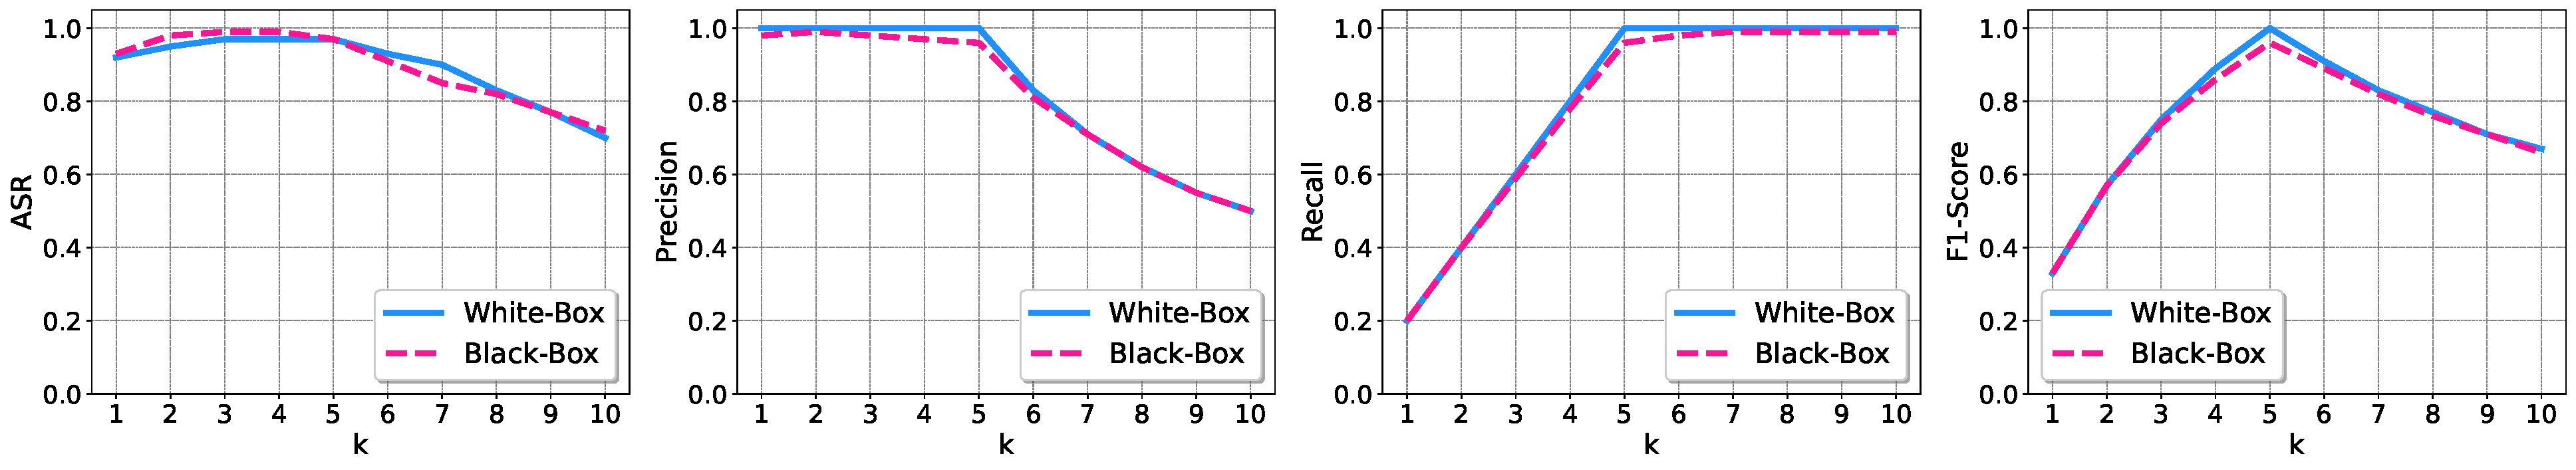
\includegraphics[width=0.9\textwidth]{figs/Impact-Of-k.pdf}}
\vspace{-3mm}
\caption{Impact of $k$ for {\name} on NQ. Figures~\ref{Impact-Of-k-HotpotQA},~\ref{Impact-Of-k-MSMARCO} (in Appendix) show results of other datasets.}
\label{Impact-Of-k}
\vspace{-4mm}
\end{figure*}

\myparatight{{\name} is computationally efficient} Table~\ref{tab:efficiency} shows the average \#Queries and runtime of {\name}. 
We have two key observations. First, on average, {\name} only needs to make around 2 queries to the GPT-4 to craft each malicious text. Second, it takes far less than 1 second for {\name} to optimize the malicious text in the black-box setting. The reason is that {\name} directly concatenates the text generated by an LLM and the target question to craft a malicious text. Further, it takes less than 30 seconds to optimize each malicious text in the white-box setting. We note that {\name} could craft malicious texts in parallel. 


\begin{table}[!t]\renewcommand{\arraystretch}{1.2}
\setlength{\tabcolsep}{1mm}
\fontsize{7.5}{8}\selectfont
\centering
\caption{Impact of retriever in RAG on {\name}.}
\vspace{-2mm}
\begin{tabular}{|c|c|c|c|c|c|c|c|}
\hline
 \multirow{2}{*}{Dataset} & \multirow{2}{*}{Attack} & \multicolumn{2}{c|}{Contriever} & \multicolumn{2}{c|}{\makecell{Contriever-ms}} & \multicolumn{2}{c|}{ANCE}   \\ \cline{3-8}
& &ASR&F1-Score&ASR&F1-Score&ASR&F1-Score \\ \hline
                      

\multirow{3}{*}{NQ} & \makecell{{\name}\\ (Black-Box)}         & 0.97& 0.96& 0.96 &0.98 & 0.95 & 0.96\\ \cline{2-8}
& \makecell{{\name}\\ (White-Box)}     & 0.97 & 1.0& 0.97 & 1.0 & 0.98 & 0.97 \\ \hline \hline 
\multirow{3}{*}{\makecell{Hotpot\\QA}} & \makecell{{\name}\\ (Black-Box)}         &   0.99 & 1.0   & 1.0  & 1.0  &  1.0 & 1.0\\ \cline{2-8}
& \makecell{{\name}\\ (White-Box)}         &   0.94 & 1.0   &  0.95 & 1.0  &  1.0 & 1.0\\ \hline \hline 
\multirow{3}{*}{\makecell{MS-\\MARCO}} & \makecell{{\name}\\ (Black-Box)}         &   0.91 & 0.89   &  0.83 & 0.91  &  0.87 & 0.91\\ \cline{2-8}
& \makecell{{\name}\\ (White-Box)}          &   0.90 & 0.94   & 0.93  & 0.99  & 0.87  & 0.90\\ \hline 

\end{tabular}
\label{tab:impact-of-retrievers}
\vspace{-4mm}
\end{table}

\myparatight{{\name} outperforms baselines}\RV{Table~\ref{tab:comparision-baseline} compares {\name} with baselines under the default setting. We have the following observations. First, {\name} outperforms those baselines, demonstrating the effectiveness of {\name}. The reason is that those baselines are not designed to simultaneously achieve retrieval and generation conditions.
Second, prompt injection attack also achieves a non-trivial ASR, although it is worse than {\name}. The reason is that, inspired by {\name} in the black-box setting, we also add the target question to the malicious texts crafted by prompt injection attacks. As a result, some malicious texts crafted by prompt injection attacks could be retrieved for the target questions as reflected by a non-trivial F1-Score. As LLMs are good at following instructions, prompt injection attack achieves a non-trivial ASR.  Note that the key difference between {\name} and prompt injection attack is that {\name} relies on malicious knowledge instead of instructions to mislead LLMs. Third, the disinformation attack (a variant of {\name}) also achieves a non-trivial ASR as some crafted malicious texts by this attack can also be retrieved (reflected by a non-trivial F1-Score). The reason is that those malicious texts are relevant to the target question. Fourth, Naive Attack, Corpus Poisoning Attack, and GCG Attack are ineffective because they cannot achieve generation, generation, and retrieval condition, respectively. } 

%\vspace{-2mm}
\subsection{Ablation Study}
We study the impact of hyperparameters on  {\name}. 
For space reasons, we defer the results for different LLMs used in RAG to Appendix~\ref{impact-of-hyperparameters-of-different-LLMs}. 
\vspace{-2mm}
\subsubsection{Impact of Hyperparameters in RAG}
\vspace{-2mm}
\myparatight{Impact of retriever}Table~\ref{tab:impact-of-retrievers} shows the effectiveness of {\name} for different retrievers under the default setting. Our results demonstrate that {\name} is consistently effective for different retrievers. {\name} is effective in the black-box setting because the crafted malicious texts are semantically similar to the target questions. Thus, they are very likely to be retrieved for the target questions by different retrievers, e.g., F1-Score is consistently high. 

\myparatight{Impact of $k$} Figure~\ref{Impact-Of-k} shows the impact of $k$. We have the following observations. First, ASR of {\name} is high when $k \leq N$ ($N=5$ by default).
The reason is that most of the retrieved texts are malicious ones when $k\leq N$, e.g., Precision (measure the fraction of retrieved texts that are malicious ones) is very high and Recall increases as $k$ increases. When $k>N$, ASR (or Precision) decreases as $k$ increases. The reason is that $(k-N)$ retrieved texts are clean ones as the total number of malicious texts for each target question is $N$. Note that Recall is close to $1$ when $k>N$, which means almost all malicious texts are retrieved for target questions.






\begin{table}[!t]\renewcommand{\arraystretch}{1.2}
\setlength{\tabcolsep}{1mm}
\fontsize{7.5}{8}\selectfont
\centering
\caption{Impact of similarity metric.}
\vspace{-2mm}
\begin{tabular}{|c|c|c|c|c|c|}
\hline
\multirow{2}{*}{Dataset} & \multirow{2}{*}{Attack} & \multicolumn{2}{c|}{Dot Product} & \multicolumn{2}{c|}{Cosine}    \\ \cline{3-6}
& &ASR&F1-Score&ASR&F1-Score \\ \hline
\multirow{2}{*}{NQ}& {\name} (Black-Box)      & 0.97 &0.96 & 0.99 & 0.96  \\ \cline{2-6}
& {\name} (White-Box)        &0.97 & 1.0& 0.97 & 0.92\\ \hline \hline 
\multirow{2}{*}{HotpotQA}& {\name} (Black-Box)      &  0.99 & 1.0  & 1.0 & 1.0  \\ \cline{2-6}
& {\name} (White-Box)          &  0.94 & 1.0  & 0.96 & 1.0 \\ \hline \hline 
\multirow{2}{*}{MS-MARCO}& {\name} (Black-Box)      &  0.91 & 0.89  & 0.93 & 0.93  \\ \cline{2-6}
& {\name} (White-Box)          &  0.90 & 0.94  & 0.83 & 0.76 \\ \hline 

\end{tabular}
\label{tab:impact-of-similarity}
\vspace{-2mm}
\end{table}



\begin{figure*}[!t]
\centering
{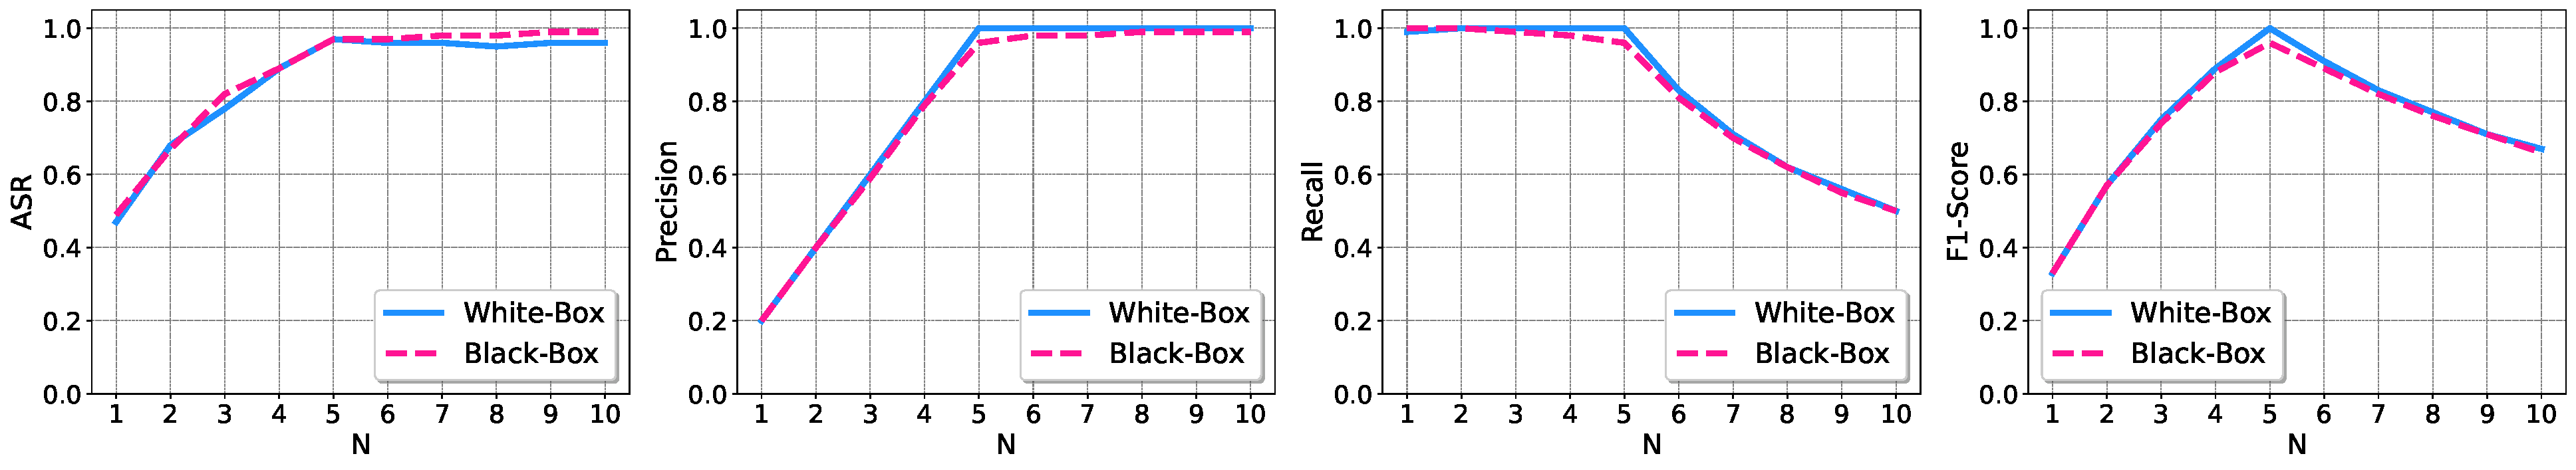
\includegraphics[width=0.9\textwidth]{figs/Impact-Of-N.pdf}}
\vspace{-3mm}
\caption{Impact of $N$ for {\name} on NQ. Figures~\ref{Impact-Of-N-HotpotQA},~\ref{Impact-Of-N-MSMARCO} (in Appendix) show results of other datasets.}
\label{Impact-Of-N}
\vspace{-3mm}
\end{figure*}





\begin{figure}[!t]
\centering
{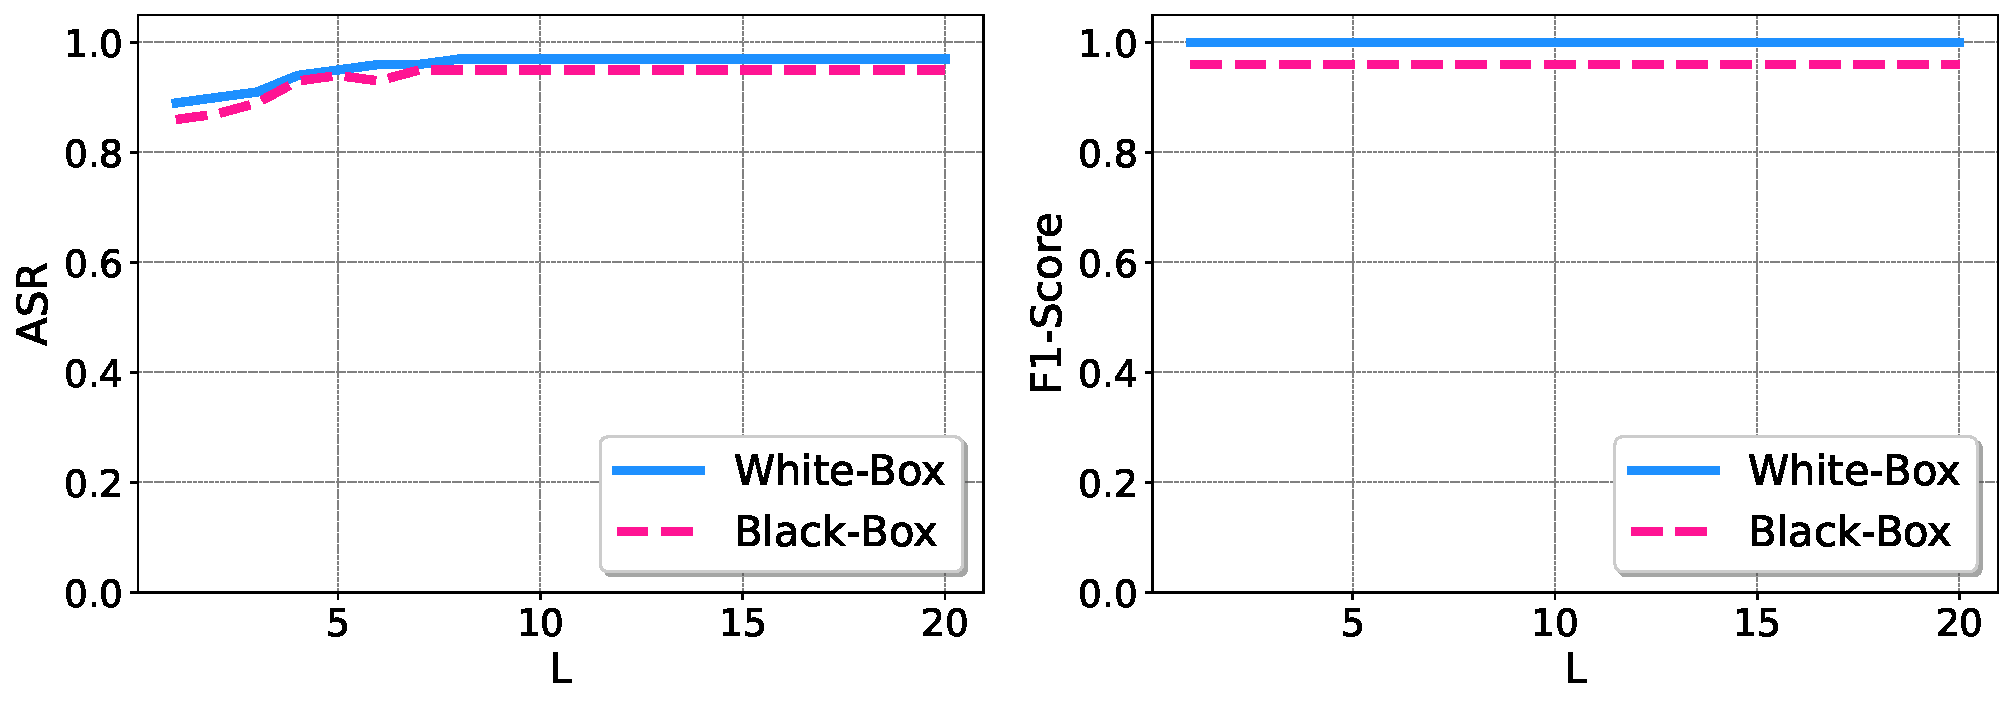
\includegraphics[width=0.45\textwidth]{figs/Impact-Of-L-20.pdf}}
\vspace{-3mm}
\caption{Impact of the number of trials $L$ in generating $I$. Figures~\ref{Impact-Of-L-20-hotpotqa},~\ref{Impact-Of-L-20-msmarco} (in Appendix) show results of other datasets.}
\label{Impact-Of-L}
\vspace{-4mm}
\end{figure}


\myparatight{Impact of similarity metric}Table~\ref{tab:impact-of-similarity} shows the results when we use different similarity metrics to calculate the similarity of embedding vectors when retrieving texts from a knowledge database for a question. We find that {\name} achieves similar results for different similarity metrics in both settings. 










\myparatight{Impact of LLMs}Table~\ref{tab:main-results} also shows the results of {\name} for different LLMs in RAG. We find that {\name} consistently achieves high ASRs. \RV{We also study the impact of the temperature hyperparameter of the LLM in RAG on {\name}. Table~\ref{tab:ablation-llm-tmp-results} in Appendix shows the results when setting a large temperature, which demonstrate that the effectiveness of {\name} is unaffected by the randomness in the decoding process of the LLM.}


\subsubsection{Impact of Hyperparameters in {\name}}
\vspace{-2mm}
\myparatight{Impact of $N$}Figure~\ref{Impact-Of-N} shows the impact of $N$. We have the following observations. First, ASR increases as $N$ increases when $N \leq k$ ($k=5$ by default). The reason is that more malicious texts are injected for each target question when $N$ is larger, and thus the retrieved texts for the target question contain more malicious ones, e.g., Precision increases as $N$ increases and Recall is consistently high. When $N>k$, ASR (or Precision) becomes stable and is consistently high. We note that Recall decreases as $N$ increases when $N>k$. The reason is that at most $k$ malicious texts could be retrieved. F1-Score measures a tradeoff between Precision and Recall, which first increases and then decreases. 





\myparatight{Impact of length $V$ in generating $I$} To achieve the generation condition, we use an LLM to generate $I$ with length $V$ (a hyperparameter) such that RAG would generate an attacker-chosen target answer for a target question. We study the impact of $V$ on the effectiveness of {\name}. Figure~\ref{Impact-Of-Text-Length}~-~\ref{Impact-Of-Text-Length-MSMARCO} (in Appendix) shows the experimental results. We find that {\name} achieves similar ASR, Precision, Recall, and F1-Score, which means {\name} is insensitive to $V$. 


\myparatight{Impact of the number of trials $L$ in generating $I$}Figure~\ref{Impact-Of-L} shows the impact of number of trials $L$ on {\name} for NQ. We find that {\name} could achieve high ASRs even when $L=1$ (i.e., one trial is made). As $L$ increases, the ASR first increases and then becomes saturated when $L \geq 10$. Our experimental results demonstrate that a small $L$ (i.e., 10) is sufficient for {\name} to achieve high ASRs. 


\myparatight{Impact of concatenation order of $S$ and $I$} By default, we concatenate $S$ and $I$ as $S \oplus I$ to craft a malicious text. We study whether the concatenation order of $S$ and $I$ would influence the effectiveness of {\name}. Table~\ref{tab:impact-of-the-order} shows the experimental results, which demonstrate that {\name} is also effective when we change their order. 

\myparatight{The effectiveness of each attack component} \RV{The effectiveness of our {\name} depends on 1) whether malicious texts are retrieved, and 2) whether the retrieved malicious texts can make the LLM in RAG generate target answers. We independently evaluate the effectiveness of each part. Table~\ref{tab:eval-of-retrieval} (in Appendix) shows the first part results, demonstrating most malicious texts are retrieved for corresponding target questions. To study the second part, we vary the number of malicious texts (randomly selected) in the $k$ retrieved texts. Table ~\ref{tab:eval-of-effectiveness-of-poisonedrag} (in Appendix) shows the results. As we can see, the ASR increases as as the number of malicious texts increases. When the number of malicious texts is small, the ASR does not reach 100\%. We suspect the reason is that most of the $k$ ($k=5$ by default) retrieved texts are clean ones, making the attack less effective, i.e., the LLM could still generate answers based on clean texts for some target questions. By contrast, when the number of malicious texts is larger than 3 (most of the $k$ retrieved texts are malicious ones), the ASR is very high.  }





\begin{table}[!t]\renewcommand{\arraystretch}{1.2}
\setlength{\tabcolsep}{1mm}
\fontsize{7.5}{8}\selectfont
\centering
\caption{Impact of the concatenation order of $S$ and $I$. }
\vspace{-2mm}
\begin{tabular}{|c|c|c|c|c|c|}
\hline
 \multirow{2}{*}{Dataset} & \multirow{2}{*}{Attack} & \multicolumn{2}{c|}{$S\oplus I$} & \multicolumn{2}{c|}{$I\oplus S$}    \\ \cline{3-6}
& &ASR&F1-Score&ASR&F1-Score \\ \hline

\multirow{2}{*}{NQ}& {\name} (Black-Box)       & 0.97 &0.96 &0.96 & 0.95 \\ \cline{2-6}
& {\name} (White-Box)      & 0.97 &1.0 & 0.95 & 1.0 \\ \hline \hline 
\multirow{2}{*}{HotpotQA}& {\name} (Black-Box)       &    0.99 & 1.0   &  0.96 & 1.0\\ \cline{2-6}
& {\name} (White-Box)      &    0.94 & 1.0   & 0.91  & 1.0\\ \hline \hline 
\multirow{2}{*}{MS-MARCO}& {\name} (Black-Box)       &    0.91 & 0.89   & 0.94  & 0.86\\ \cline{2-6}
& {\name} (White-Box)      &    0.90 & 0.94   &  0.92 & 0.99\\ \hline 
\end{tabular}
\label{tab:impact-of-the-order}
\vspace{-3mm}
\end{table}


\begin{table}[!t]\renewcommand{\arraystretch}{1.2}
\setlength{\tabcolsep}{1mm}
\fontsize{7.5}{8}\selectfont 
\centering
\caption{Impact of adversarial example method on {\name} in white-box setting.}
\vspace{-2mm}
\begin{tabular}{|c|c|c|c|c|}
\hline
\multirow{2}{*}{Dataset} & \multicolumn{2}{c|}{HotFlip} & \multicolumn{2}{c|}{TextFooler} \\ \cline{2-5}
&ASR &F1-Score &ASR &F1-Score  \\ \hline
                      
\multirow{1}{*}{NQ}       & 0.97 & 1.0  & 0.93 & 0.91  \\ \cline{2-5} \hline 
\multirow{1}{*}{HotpotQA} & 0.94 & 1.0  & 0.98 & 0.99  \\ \cline{2-5} \hline 
\multirow{1}{*}{MS-MARCO} & 0.90 & 0.94 & 0.84 & 0.84  \\ \cline{2-5} \hline 

\end{tabular}
\label{tab:textfooler}
\vspace{-5mm}
\end{table}


\begin{table*}[!t]\renewcommand{\arraystretch}{1.2}
\setlength{\tabcolsep}{1mm}
\fontsize{7.5}{8}\selectfont
\centering
\caption{\RV{The effectiveness of {\name} when using less powerful LLMs to generate $I$ to achieve generation condition.}}
\vspace{-2mm}
\begin{tabular}{|c|c|c|c|c|c|c|c|c|c|c|}
\hline
 \multirow{2}{*}{Dataset} & \multirow{2}{*}{Attack} & \multicolumn{2}{c|}{PaLM 2} & \multicolumn{2}{c|}{\makecell{GPT-3.5}} & \multicolumn{2}{c|}{LLaMa-2-7B}& \multicolumn{2}{c|}{Vicuna-7B}   \\ \cline{3-10}
& &ASR&F1-Score&ASR&F1-Score&ASR&F1-Score&ASR&F1-Score \\ \hline
                      

 \multirow{2}{*}{NQ} & {\name} (Black-Box) & 0.99 & 0.97 & 0.98 & 0.95  & 0.92 & 0.93 & 0.95 & 0.95 \\ \cline{2-10}
 & {\name} (White-Box) & 0.97 & 1.00 & 0.98 & 0.99  & 0.91 & 0.98 & 0.97 & 0.99  \\ \hline \hline 

 \multirow{2}{*}{HotpotQA} & {\name} (Black-Box) & 0.97 & 1.00 & 0.99 & 1.00 &  0.96 & 0.99 & 0.98 & 1.00 \\ \cline{2-10}
 & {\name} (White-Box) & 0.96 & 1.00 & 0.96 & 1.00 &  0.97 & 1.00 & 0.99 & 1.00  \\ \hline \hline 

 \multirow{2}{*}{MS-MARCO} & {\name} (Black-Box) & 0.91 & 0.88 & 0.89 & 0.84 &  0.79 & 0.80 & 0.90 & 0.82 \\ \cline{2-10}
 & {\name} (White-Box) & 0.95 & 0.97 & 0.89 & 0.95 &  0.84 & 0.89 & 0.92 & 0.95  \\ \hline 

\end{tabular}
\label{tab:impact-of-llm}
\vspace{-4mm}
\end{table*}

\begin{table}[!t]\renewcommand{\arraystretch}{1.5}
\setlength{\tabcolsep}{1mm}
\fontsize{7.5}{8}\selectfont
\centering
\caption{\RV{The effectiveness of {\name} under advanced RAG.}}
\vspace{-2mm}
\begin{tabular}{|c|c|c|c|c|c|}
\hline
 \multirow{2}{*}{Dataset} & \multirow{2}{*}{Attack}  & \multicolumn{2}{c|}{\makecell{Self-RAG~\cite{asai2023self}}} & \multicolumn{2}{c|}{CRAG~\cite{yan2024corrective}}   \\ \cline{3-6}
& &ASR&F1-Score&ASR&F1-Score \\ \hline
                      
\multirow{2}{*}{NQ} 
& \makecell{{\name} (Black-Box)}         & 0.77 & 0.96 & 0.78 & 0.96\\ \cline{2-6}
& \makecell{{\name} (White-Box)}         & 0.74 & 1.0 & 0.82 & 1.0 \\ \hline \hline 
\multirow{2}{*}{\makecell{Hotpot\\QA}} 
& \makecell{{\name} (Black-Box)}         & 0.87 & 1.0 & 0.76 & 1.0\\ \cline{2-6}
& \makecell{{\name} (White-Box)}         & 0.79 & 1.0 & 0.70 & 1.0\\ \hline \hline 
\multirow{2}{*}{\makecell{MS-\\MARCO}} 
& \makecell{{\name} (Black-Box)}         & 0.73 & 0.89 & 0.74 & 0.89\\ \cline{2-6}
& \makecell{{\name} (White-Box)}         & 0.75 & 0.94 & 0.72 & 0.94\\ \hline 

\end{tabular}
\label{tab:advanced-rag}
\vspace{-3mm}
\end{table}



\myparatight{Impact of adversarial text generation methods in generating $S$ to achieve retrieval condition} In the white-box setting, {\name} can utilize any existing adversarial  text generation methods~\cite{ebrahimi2018hotflip,jin2020bert} 
to optimize $S$ in Equation~\ref{white-box-opt}. 
By default, we use HotFlip~\cite{ebrahimi2018hotflip}. Here we also evaluate the effectiveness of {\name} when using TextFooler~\cite{jin2020bert}, which 
replaces words with their synonyms to keep semantic meanings. \RV{Table~\ref{tab:textfooler} shows the results, which demonstrate that {\name} could achieve very high ASR and F1-Score using both methods. We also compare the computational overhead of the two methods in Table~\ref{tab:overhead} (in Appendix). We find that {\name} could incur higher computational overhead using TextFooler. The reason is that TextFooler aims to keep the semantic meaning when crafting adversarial texts (e.g., using synonyms of words for replacement in optimizing adversarial text). As a result, the candidate word space in each iteration is smaller, which means more iterations are needed for optimization, resulting in higher overhead. However, the adversarial text crafted by TextFooler is more stealthy as it keeps semantics. Our results demonstrate that there is a tradeoff between computational overhead and stealthiness.}

\myparatight{Impact of the LLM in generating $I$ to achieve generation condition}
\RV{By default, we use GPT-4 to generate $I$ to achieve the generation condition because it is very powerful. We also evaluate whether {\name} could be effective when using less powerful LLMs to generate $I$. As those LLMs are less powerful, we utilize in-context learning~\cite{brown2020language} to improve the performance (we provide two demonstration samples to the LLM, please see Appendix~\ref{appendix-less-powerful-LLM-for-I} for details).
Table~\ref{tab:impact-of-llm} shows the experimental results under the default setting, which show our {\name} is also effective when using less powerful LLMs to generate $I$ with in-context learning.}


\vspace{-3mm}
\section{Evaluation for Real-world Applications}
\vspace{-2mm}
We evaluate {\name} for more sophisticated RAG schemes and two real-world applications, including Wikipedia-based ChatBot and LLM agents.

\vspace{-3mm}
\subsection{Advanced RAG Schemes}
\RV{In our above experiment, we mainly focus on basic RAG. However, the basic RAG scheme might be insufficient for more complex real-world applications. To this end, many advanced RAG schemes~\cite{asai2023self, yan2024corrective, yoran2023making, luo2023search, zhang2024raft} were proposed to improve the performance of the basic RAG scheme. 
For example, Asai et al.~\cite{asai2023self} introduced Self-RAG, which trains an LLM that can adaptively use the retrieved contexts on-demand and reflect on its own generations to enhance the factuality and quality of generated answers. Yan et al.~\cite{yan2024corrective} proposed CRAG, which uses a lightweight retrieval evaluator to assess the quality (e.g., relevance of retrieved texts to questions) of retrieved contexts, thus enhancing the robustness and correctness of RAG. 
Roughly speaking, their key idea is to enhance the relevance of the retrieved texts and thus make the LLM more likely to generate correct answers based on the retrieved texts. We conduct experiments to evaluate the effectiveness of {\name} for these advanced RAG schemes. Table~\ref{tab:advanced-rag} shows {\name} can achieve high ASRs, demonstrating that those advanced RAG schemes are also vulnerable to our {\name}. The reason is that the crafted malicious texts are relevant to the target questions, making the LLM generate incorrect answers based on malicious texts. 
}






\vspace{-4mm}
\subsection{Wikipedia-based ChatBot}
\vspace{-2mm}
In our threat model, we consider an attacker can inject malicious texts into a knowledge database collected from Wikipedia by maliciously editing Wikipedia articles~\cite{carlini2023poisoning}.
We use a case study to evaluate the effectiveness of {\name} in this scenario. 
We used the English Wikipedia dump from Dec. 20, 2018 to create a knowledge database~\cite{karpukhin2020dense}. In particular, each English Wikipedia article (non-text parts are removed) is split into disjoint texts of 100 words. The total number of texts in the knowledge database is 21,015,324. We create a ChatBot based on this knowledge database using the same system prompt as in Appendix~\ref{appendix-sec-system-prompt}. We evaluate whether our {\name} is effective for this large knowledge database. 
We use the default setting of our previous evaluation (in Section~\ref{exp:setup-exp}). We reuse the target questions from our previous three datasets (i.e., NQ, HotpotQA, and MS-MARCO) and inject five malicious texts for each target question. Results in Table~\ref{tab:real-world case study} show {\name} is effective in this real-world scenario. 


\begin{table}[!t]\renewcommand{\arraystretch}{1.5}
\setlength{\tabcolsep}{1mm}
\fontsize{7.5}{8}\selectfont 
\centering
\caption{{\name} is still effective in a real-world scenario, where the knowledge database consists of 21,015,324 texts from Dec. 20, 2018 Wikipedia dump.}
\vspace{-2mm}
\begin{tabular}{|c|c|c|c|}
\hline
  \makecell{Dataset of \\Target Questions} &{Attack} & ASR&F1-Score\\ \hline
                      
\multirow{2}{*}{NQ}& {\name} (Black-Box)         & 0.95 & 0.95  \\ \cline{2-4}
& {\name} (White-Box)         & 0.97 & 0.99 \\ \hline \hline 
\multirow{2}{*}{HotpotQA}& {\name} (Black-Box)            & 1.0 & 1.0  \\ \cline{2-4}
& {\name} (White-Box)           & 0.94 & 1.0 \\ \hline \hline 
\multirow{2}{*}{MS-MARCO}& {\name} (Black-Box)          & 0.94 & 0.95 \\ \cline{2-4}
& {\name} (White-Box)        & 0.91 & 0.98  \\ \hline 

\end{tabular}
\label{tab:real-world case study}
\vspace{-3mm}
\end{table}

\subsection{LLM Agent}
We also evaluate {\name} for LLM agents that interact with an external environment to obtain information for a task. We adopt the ReAct Agent framework~\cite{yao2022react}, which combines reasoning and acting with LLMs. Given a question-answering task, the agent will perform a sequence of thought-action-observation steps to solve the task. The action space consists of two actions in our experiments: document retrieval and task finishing. For document retrieval, the agent will retrieve $k$ documents from a knowledge database (i.e., interacting with an environment to obtain information). For task finishing, the agent finishes the question-answering task and outputs the final answer. In each thought-action-observation step, the agent first generates a thought and an action. The thought provides a verbal reasoning processing for the next action (e.g., ``I need to search Chicago Fire Season 4 and find how many episodes it has.'') to solve a task. Then, the agent takes the generated action (e.g., ``Search [Chicago Fire Season 4]'') to obtain additional information (i.e., observation). Based on the additional information, the agent performs the next thought-action-observation step. This process is repeated until the task is finished (output final answer for the question-answering task) or a maximum number of steps is reached. We use the open-sourced code~\cite{yao2022react} in our experiment.  We use the default setting of the previous evaluation and conduct the experiment on NQ, HotpotQA and MS-MARCO datasets. Our black-box attack achieves 0.72, 0.58, and 0.52 ASR, respectively.




